\subsection{Likelihood estimator using self-adapting phase-space binning (PDE-Foam)}
\label{sec:pdefoam}

The PDE-Foam\index{PDE-Foam, multi-dimensional likelihood} 
method~\cite{pdefoam} is an extension of PDE-RS, which
divides the multi-dimensional phase space in a finite number of
hyper-rectangles (cells) of constant event density.  This ``foam'' of
cells is filled with averaged probability density information sampled
from the training data.  For a given number of cells, the
binning algorithm adjusts the size and position of the cells inside
the multi-dimensional phase space based on a binary split algorithm that
minimises the variance of the event density in the cell.  The binned
event density information of the final foam is stored in cells,
organised in a binary tree, to allow a fast and memory-efficient
storage and retrieval of the event density information necessary for
classification or regression.  The implementation of PDE-Foam is based on the
Monte-Carlo integration package TFoam~\cite{tfoam} included in ROOT.

In classification mode PDE-Foam forms bins of similar density of signal 
and background events or the ratio of signal to background. In regression 
mode the algorithm determines cells with small varying regression targets. 
In the following, we use the term density ($\rho$) for the event density in
case of classification or for the target variable density in case of
regression.

\subsubsection{Booking options}

The PDE-Foam classifier is booked via the command:
\begin{codeexample}
\begin{tmvacode}
factory->BookMethod( Types::kPDEFoam, "PDEFoam", "<options>" );
\end{tmvacode}
\caption[.]{\codeexampleCaptionSize Booking of PDE-Foam: the first 
         argument is a predefined enumerator, the second argument is a
	 user-defined string identifier, and the third argument is the
	 configuration options string.  Individual options are
	 separated by a ':'.  See Sec.~\ref{sec:usingtmva:booking} for
	 more information on the booking.}
\end{codeexample}
%
The configuration options for the PDE-Foam method are summarised in 
Option Table~\ref{opt:mva::pdefoam}.

% ======= input option table ==========================================
\begin{option}[p]
\input optiontables/MVA__PDEFoam.tex
\caption[.]{\optionCaptionSize Configuration options reference for MVA
  method: {\em PDE-Foam}.  The options in Option
  Table~\ref{opt:mva::methodbase} on
  page~\pageref{opt:mva::methodbase} can also be configured.  }
\label{opt:mva::pdefoam}
\end{option}
% =====================================================================

Table~\ref{tab:opt-combinations} gives an overview of supported
combinations of configuration options.

\begin{table}[th]
\centering
\renewcommand{\checkmark}{\YES}
\setlength{\tabcolsep}{0.0pc}
{\small
\begin{tabular*}{\textwidth}{@{\extracolsep{\fill}}lcccc} 
\hline
&&&&\\[\BD]
                 &    \multicolumn{2}{c}{Classification}     & \multicolumn{2}{c}{Regression} \\
  Option         & Separated foams & Single foam             & Mono target  & Multi target \\
&&&&\\[\BD]                                       
\hline                                                 
&&&&\\[\BD]                                       
  \code{SigBgSeparate}  & True            & False                   & --           & -- \\
  \code{MultiTargetRegression} & --       & --                      & False        & True \\
&&&&\\[\BD]                                       
\hline                                                 
&&&&\\[\BD]                                       
  \code{Kernel}         & \checkmark      & \checkmark              & \checkmark   & \checkmark \\
  \code{TargetSelection} & \NO             & \NO                      & \NO           & \checkmark \\
  \code{TailCut}        & \checkmark      & \checkmark              & \checkmark   & \checkmark \\
  \code{UseYesNoCell}   & \checkmark      & \checkmark              & \NO          & \NO \\
  \code{MaxDepth}       & \checkmark      & \checkmark              & \checkmark   & \checkmark \\
&&&&\\[\BD]                                       
\hline                                                 
\end{tabular*}
}
\caption[.]{\captionfont Availability of options for the two classification and 
            two regression modes of PDE-Foam. Supported options are marked by a 
            '\checkmark', while disregarded ones are marked by a '\NO'.}
\label{tab:opt-combinations}
\end{table}

\subsubsection{Description and implementation of the foam algorithm}
\label{sec:foam-algorithm}
Foams for an arbitrary event sample are formed as follows.

\begin{enumerate}
  \item \emph{Setup of binary search trees}. A binary search tree is
    created and filled with the $d$-dimensional event tuples form the 
    training sample as for the PDE-RS method (\cf Sec.~\ref{sec:pders}).

  \item \emph{Initialisation phase}. A foam is created, which at first
    consists of one $d$-dimensional hyper-rectangle (base cell).  The
    coordinate system of the foam is normalised such that the base
    cell extends from 0 to 1 in each dimension. The coordinates of the
    events in the corresponding training tree are linearly transformed
    into the coordinate system of the foam.

  \item \emph{Growing phase}. A binary splitting algorithm iteratively
    splits cells of the foam along axis-parallel hyperplanes until the maximum
    number of active cells (set by \code{nActiveCells}) is reached.
    The splitting algorithm minimises the relative variance of the
    density $\sigma_{\rho}/\langle\rho\rangle$ across each cell (\cf
    Ref.~\cite{tfoam}).  For each cell \code{nSampl} random points
    uniformly distributed over the cell volume are generated. For each
    of these points a small box centred around this point is defined.
    The box has a size of \code{VolFrac} times the size of the base
    cell in each dimension.  The density is estimated as the number of
    events contained in this box divided by the volume of the box.\footnote
    {
       In case of regression this is the average target value computed 
       according to Eq.~(\ref{eq:PDERSregratio}), page~\pageref{eq:PDERSregratio}.
    }  
    The densities obtained for all sampled points in the cell are
    projected onto the $d$ axes of the cell and the projected values are
    filled in histograms with \code{nBin} bins.  The next cell to be
    split and the corresponding division edge (bin) for the split
    are selected as the ones that have the largest relative variance.
    The two new daughter cells are marked as `active' cells and the
    old mother cell is marked as `inactive'.  A detailed description
    of the splitting algorithm can be found in Ref.~\cite{tfoam}.  The
    geometry of the final foam reflects the distribution of the
    training samples: phase-space regions where the density is
    constant are combined in large cells, while in regions with large
    density gradients many small cells are created. 
    Figure~\ref{fig:pdefoam-foam-nokernel} displays a foam obtained 
    from a two-dimensional Gaussian-distributed training sample.

  \item \emph{Filling phase}. Each active cell is filled with values
    that classify the event distribution within this cell and which permit
    the calculation of the classification or regression discriminator. 

  \item \emph{Evaluation phase}. The estimator for a given event is
    evaluated based on the information stored in the foam cells. The
    corresponding foam cell, in which the event variables
    ($d$-dimensional vector) of a given event is contained, is determined
    with a binary search algorithm.\footnote
    {
       For an event that falls outside the foam boundaries, the cell with the smallest 
       Cartesian distance to the event is chosen.
    }
\end{enumerate}

\begin{figure}[t]
\centering
   \subfigure[foam projection without kernel]{%
      \label{fig:pdefoam-foam-nokernel}
      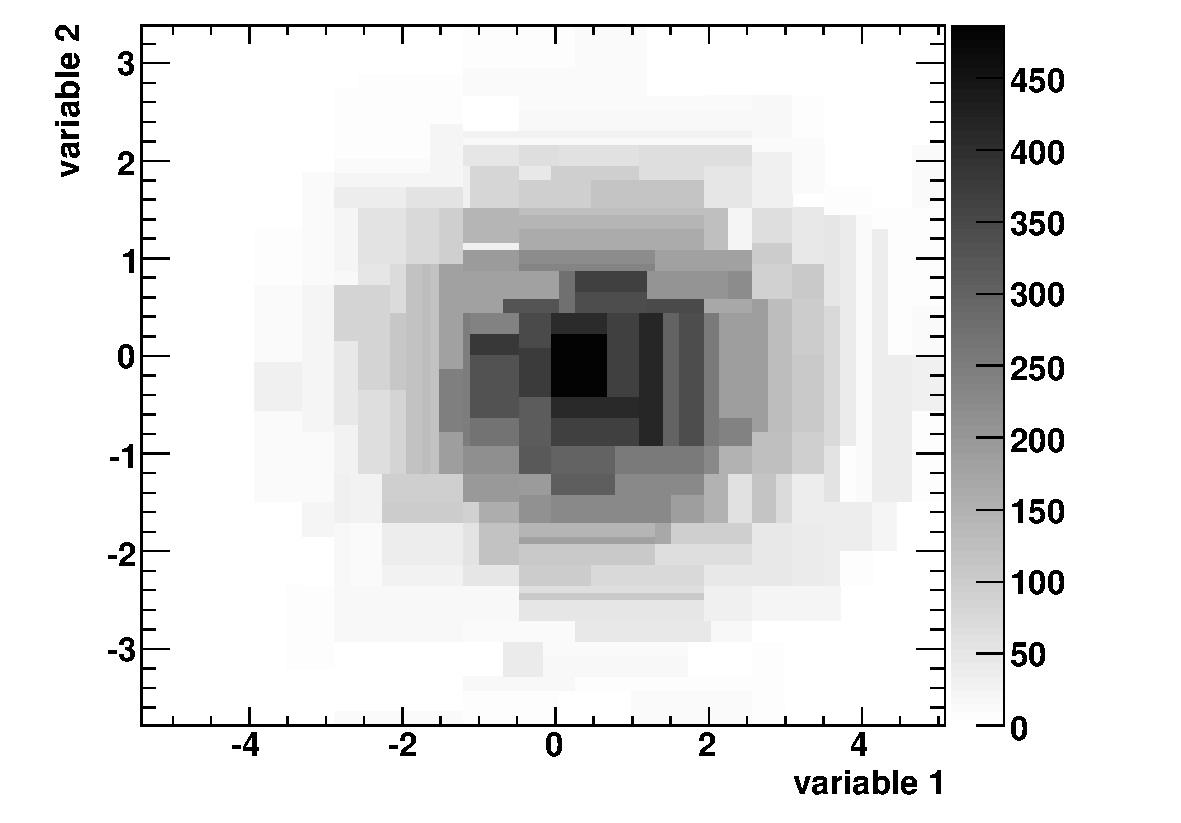
\includegraphics[width=0.48\textwidth,clip]{plots/PDEFoam-foam_bw}}
   \subfigure[foam projection with Gaussian kernel]{%
      \label{fig:pdefoam-foam-kernel}
      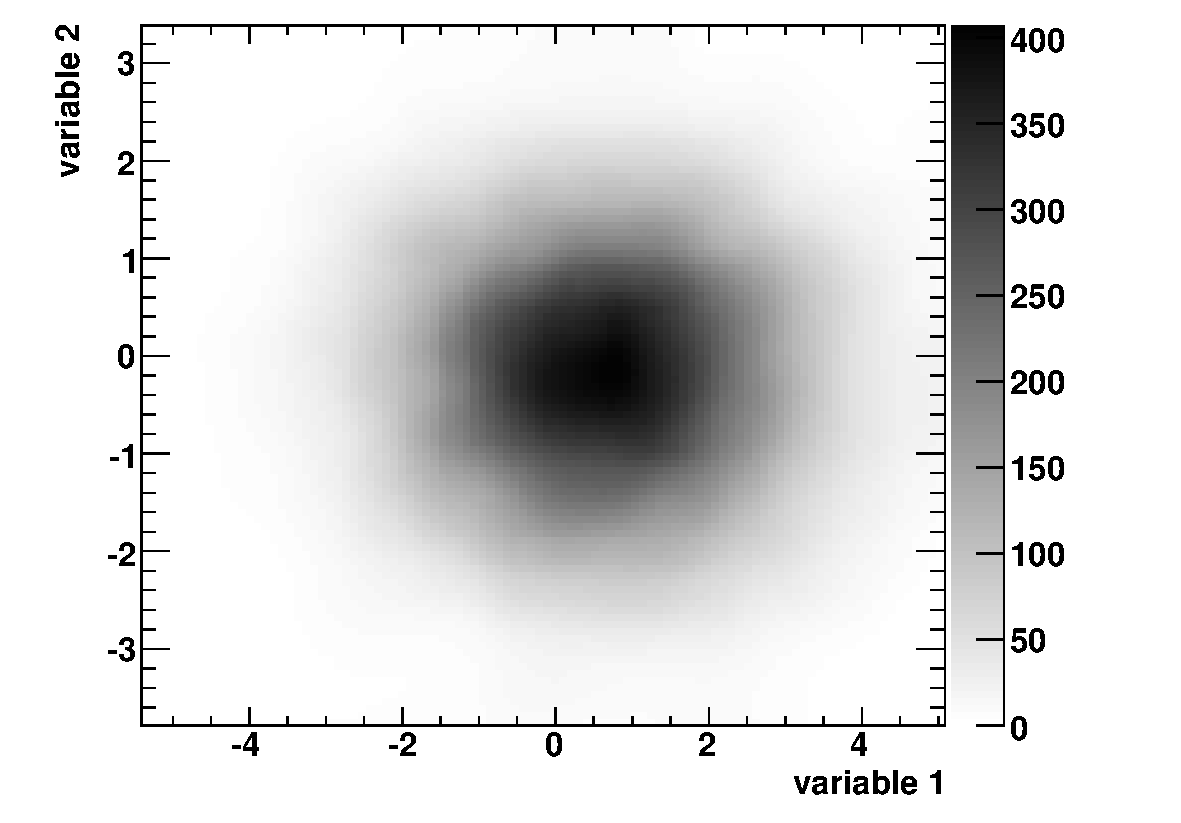
\includegraphics[width=0.48\textwidth,clip]{plots/PDEFoam-foam_kernel_bw}}
\caption[.]{Projections of a two-dimensional foam with 500 cells 
    for a Gaussian distribution on a two-dimensional histogram. The foam
    was created with 5000 events from the input tree. (a) shows the
    reconstructed distribution without kernel weighting and (b)
    shows the distribution weighted with a Gaussian kernel.  The grey shades
    indicate the event density of the drawn cell.  For more details
    about the projection function see the description on page
    \pageref{sec:pdefoam-visualise}.}
\label{fig:pdefoam-foam}
\end{figure}

The initial trees which contain the training events and which are needed to
evaluate the densities for the foam build-up, are discarded after the
training phase.  The memory consumption for the foam is $160$ bytes
per foam cell plus an overhead of $1.4$ kbytes for the PDE-Foam object
on a $64$ bit architecture.  Note that in the foam all cells created
during the growing phase are stored within a binary tree
structure. Cells which have been split are marked as inactive and
remain empty. To reduce memory consumption, the cell geometry is
not stored with the cell, but rather obtained recursively from the
information about the division edge of the corresponding mother
cell. This way only two short integer numbers per cell represent the
information of the entire foam geometry: the division coordinate
and the bin number of the division edge.

%%%%%%%%%%%%%%%%%%%%%%%%%%%%%%%%%%%%%%%%%%%%%%%%%%%%%%%%%%%%%%%
\subsubsection*{PDE-Foam options}

\begin{itemize}
\item \code{TailCut} -- {\em boundaries for foam geometry}\\
A parameter
\code{TailCut} is used to define the geometry of the base
cell(s) such that outliers of the distributions in the training ensemble
are not included in the volume of the base cell(s). In a first
step, the upper and lower limits for each input variable are determined
from the training sample.  Upper and a lower bounds are then
determined for each input variable, such that on both sides a fraction 
\code{TailCut} of all events is excluded.
The default value of \code{TailCut = 0.001} ensures a sufficient
suppression of outliers for most input distributions. For cases where
the input distributions have a fixed range or where they are
discontinuous and/or have peaks towards the edges, it can be 
appropriate to set \code{TailCut} to 0.
Note that for event classification it is guaranteed that 
the foam has an infinite coverage: events outside the foam volume 
are assigned to the cell with the smallest Cartesian distance to the event.

\item \code{nActiveCells} -- {\em maximum number of active foam cells }\\
In most cases larger \code{nActiveCells} values result in more accurate 
foams, but also lead to longer computation time during the foam formation, 
and require more storage memory. The default value of 500
was found to be a good compromise for most practical applications if
the size of the training samples is of the order of $10^4$ events.
Note that the total number of cells, \code{nCells}, is given
as $\texttt{nCells}=\texttt{nActiveCells}\cdot 2-1$,
since the binary-tree structure of the foam requires all inactive
cells to remain part of the foam (see \emph{Growing phase}).

\item \code{VolFrac} -- {\em size of the probe volume for the density sampling of the training data}\\
The volume is defined as a $d$-dimensional box with edge length
\code{VolFrac} times the extension of the base cell in each dimension. 
The default of $1/15$ results in a box with volume $1/15^{d}$ times
the volume of the base cell. Smaller values of \code{VolFrac}
increase the sampling speed, but also make the algorithm more
vulnerable to statistical fluctuations in the training sample (overtraining).
In cases with many observables ($>5$) and small training samples ($<10^4$),
\code{VolFrac} should be increased for better classification results. 

\item \code{nSampl} -- {\em number of samplings per cell and per cell-division step }\\
The computation time for the foam formation scales
linearly with the number of samplings. The default of 2000 was found
to give sufficiently accurate estimates of the density distributions
with an acceptable computation time.\footnote
{
   Contrary to the original application where an analytical function is 
   used, increasing the number of samplings does not automatically lead to 
   better accuracy. Since the density is defined by a limited event sample, 
   it may occur that always the same event is found for all sample points.
}

\item \code{nBin} -- {\em number of bins for edge histograms }\\
The number of bins for the edge histograms used to determine the
variance of the sampled density distributions within one cell are set
with the parameter \code{nBin}. The performance in typical
applications was found to be rather insensitive to the number of bins.
The default value of 5 gives the foam algorithm sufficient flexibility
to find the division points, while maintaining sufficient statistical
accuracy also in case of small event samples.

\item \code{Nmin} -- {\em Minimal number of events for cell split}\\
If \code{Nmin} is set to a value greater than zero, the foam will only consider
cells with a number of events greater than \code{Nmin} to be split.
If no more cells are found during the growing phase for which this
condition is fulfilled, the foam will stop splitting cells, even if
the target number of cells is not yet reached. 
This option prevents
the foam from adapting to statistical fluctuations in the training
samples (overtraining). 
Note that event 
weights are not taken into account for evaluating the number of events 
in the cell. 

In particular for training samples with small event numbers of less
than $10^4$ events this cut improves the performance. The default
value of (\code{Nmin = 100}) was found to give good results in most
cases.  It should be reduced in applications
with very small training samples (less than 200 training events) and
with many cells. 

\item \texttt{Kernel} -- {\em cell weighting with kernel functions:\index{Kernel estimation}}\\
\label{sec:PDEFoam-kernel}%
A Gaussian Kernel smoothing is applied during the evaluation
phase, if the option \code{Kernel} is set to ``\code{Gauss}''.  In this
case all cells contribute to the calculation of the discriminant for a
given event, weighted with their Gaussian distance to the
event.  The average cell value $v$ (event density in case of
separated foams, and the ratio
$n_S/(n_S+n_B)$ in case of a single foam)
for a given event ${\mathbf x}=(x_1, \ldots, x_\Nvar)$ is calculated by
%
\beq
  v = \frac{\sum_{\text{all cells } i}G(D(i, \mathbf{x}), 0, \texttt{VolFrac})\cdot v_i}%
           {\sum_{\text{all cells } i}G(D(i, \mathbf{x}), 0, \texttt{VolFrac})}\,,
\eeq
%
where $v_i$ is the output value in cell $i$, 
$G(x, x_0, \sigma) = \exp(-(x-x_0)^2/2\sigma^2)$, and $D(i,\mathbf{x})$ 
is the minimal Euclidean distance between $\mathbf{x}$ and any point
$\mathbf{y}$ in cell $i$
%
\beq
  D(i, \mathbf{x}) = \min_{\mathbf{y}\in\text{cell }i}|\mathbf{x}-\mathbf{y}|\,.
\eeq
%
The Gaussian kernel avoids discontinuities of the discriminant
values at the cell boundaries.  In most cases it results in an
improved separation power between signal and background.  However, the
time needed for classification increases due to the larger number of
computations performed.  A comparison between foams with and without
Gaussian kernel can be seen in Fig.~\ref{fig:pdefoam-foam}.

A linear interpolation with adjacent cells in each dimension is applied during 
the classification phase, if the option \code{Kernel} is set to ``\code{LinNeighbors}''.
This results in faster classification than the Gauss weighting of all cells
in the foam.

\item \texttt{UseYesNoCell} -- {\em Discrete classification output}\\
  If \texttt{UseYesNoCell} is set to \texttt{False} (default), the
  discriminant \eqref{eq:PDEFoamSeparatedRatio} is returned as
  classification output.  If \texttt{UseYesNoCell} is set to
  \texttt{True}, $-1$ is returned for events with discriminant $<0.5$
  (background-like) and $+1$ is returned for events with $\geq 0.5$
  (signal-like).

\item \texttt{MaxDepth} -- {\em Maximum cell tree depth}\\
  The cell tree depth can be limited by using this option.  When
  \texttt{MaxDepth} is set to an integer value greater than zero, the
  created cell tree will not be deeper than \texttt{MaxDepth}.  By
  convention the root node has depth $1$, which implies that a foam
  with $2$ active cells ($3$ cells in total) has depth $2$.  If
  $\texttt{nActiveCells} \geq 2^{\texttt{MaxDepth}-1}$ the resulting
  cell tree will be completely balanced.  When \texttt{MaxDepth} is
  set to $0$, the cell tree depth is not limited.

\item \texttt{DTLogic} -- {\em Cell split algorithm}\\
In order to emulate a decision tree-like cell splitting algorithm, the
option \texttt{DTLogic} was introduced.  When set to
\texttt{GiniIndex}, \texttt{MisClassificationError} or
\texttt{Cross\-En\-tro\-py}, the algorithm projects all events in a
cell onto the cell edges and probes \texttt{nBin-1} division points
such that the separation gain
\begin{align}
%  \text{separation gain} = 
  \text{gain(parent cell)} -
  \text{gain(daughter cell 1)} 
  - \text{gain(daughter cell 2)}
\end{align}
is maximal (see Sec.~\ref{sec:treebuilding}).  For a given separation
type and a given cell the gain is defined as
\begin{align}
  &\texttt{GiniIndex :} & \text{gain(cell)}&=p(1-p),\\
  &\texttt{MisClassificationError :} & \text{gain(cell)}&=1-\max(p,1-p),\\
  &\texttt{CrossEntropy :} & \text{gain(cell)}&=-p\log p-(1-p)\log(1-p),
\end{align}
where $p=n_S/(n_S+n_B)$ in the considered cell.  When \texttt{DTLogic}
is set to \texttt{None} (default), the PDE-Foam cell splitting
algorithm (see Sec.~\ref{sec:foam-algorithm}) is used.  This option is
available only for classification and is an alternative to the
classification with two separate foams or one single foam (see
Sec.~\ref{sec:PDEFoam-classification}).


\item \texttt{FillFoamWithOrigWeights} -- {\em Event weights for boosting}\\
  Since the PDE-Foam cells are filled with events after the splitting,
  it is in principle possible to use different event weights for the
  filling than for the foam build-up.  The option
  \texttt{FillFoamWithOrigWeights} was created to choose either the
  original or the full event weight (including the boost weight) to be
  filled into the foam cells after the build-up.  This option is only
  relevant for boosting, because for non-boosted classifiers the boost
  weights are always $1$.  When setting
  \texttt{FillFoamWithOrigWeights=T}, one would only boost the foam
  geometry, instead of the cell content.  This would slow down the
  boosting process, because the boost weights are ignored in the
  classification.  In most cases studied
  \texttt{FillFoamWithOrigWeights=T} leads to worse classification
  results than \texttt{FillFoamWithOrigWeights=F} for the same number
  of boosts.  However, when using stronger boosting by choosing
  \texttt{AdaBoostBeta} accordingly, filling the original weights into
  the foam can improve the performance.
\end{itemize}

%%%%%%%%%%%%%%%%%%%%%%%%%%%%%%%%%%%%%%%%%%%%%%%%%%%%%%%%%%%%%%%

The PDE-Foam algorithm exhibits stable performance with respect to variations
in most of the parameter settings. However, optimisation of the parameters is required
for small training samples ($<10^4$ events) in combination with many
observables ($>5$). In such cases, \code{VolFrac} should be increased until 
an acceptable performance is reached. Moreover, in cases where the classification 
time is not critical, one of the \code{Kernel} methods should be applied
to further improve the classification performance. For large training samples ($>10^5$) 
and if the training time is not critical,
\code{nActiveCells} should be increased to improve the classification performance.

%%%%%%%%%%%%%%%%%%%%%%%%%%%%%%%%%%%%%%%%%%%%%%%%%%%%%%%%%%%

\subsubsection{Classification}
\label{sec:PDEFoam-classification}

To classify an event in a $d$-dimensional phase space as being either
of signal or of background type, a local estimator of the probability
that this event belongs to either class can be obtained from the
foam's hyper-rectangular cells. The foams are created and filled based
on samples of signal and background training events.  For
classification two possibilities are implemented. One foam can be used
to separate the S/B probability density or two separate foams are
created, one for the signal events and one for background events.

\subsubsection*{1)~Separate signal and background foams} 

If the option \code{SigBgSeparate = True} is set, the
method PDE-Foam treats the signal- and background distributions
separately and performs the following steps to form the two foams and
to calculate the classifier discriminator for a given event:

\begin{enumerate}
  \item \emph{Setup of training trees}. Two binary search trees are
    created and filled with the $d$-dimensional observable vectors of
    all signal and background training events, respectively.

  \item \emph{Initialisation phase}. Two independent foams for signal
    and background are created.

  \item \emph{Growing phase}. The growing is performed independently
    for the two foams.  The density of events is estimated as the
    number of events found in the corresponding tree that are
    contained in the sampling box divided by the volume of the box
    (see \code{VolFrac} option).  The geometries of the final foams
    reflect the distribution of the training samples: phase-space
    regions where the density of events is constant are combined in
    large cells, while in regions with large gradients in density many
    small cells are created.

  \item \emph{Filling phase}. Both for the signal and background foam
    each active cell is filled with the number of training
    events, $n_S$ (signal) or $n_B$ (background), contained in the 
    corresponding cell volume, taking into account
    the event weights $w_i$: $n_S=\sum_{\text{sig. cell}}w_i$, 
    $n_B=\sum_{\text{bg. cell}}w_i$. 

  \item \emph{Evaluation phase}. The estimator for a given event is
    evaluated based on the number of events stored in the foam
    cells. The two corresponding foam cells that contain the event are
    found.  The number of events ($n_S$ and $n_B$) is
    read from the cells.  The estimator $\RPDEFoam(i)$ is then given by
    \beq
    \label{eq:PDEFoamSeparatedRatio}
    \RPDEFoam(i) = \frac{n_{S}/V_{S}}
    {\frac{n_B}{V_B} + 
      \frac{n_S}{V_S}} \, , 
    \eeq
    where $V_S$ and $V_B$ are the respective
    cell volumes.
    The statistical error of the estimator is calculated as:
    \beq
    \label{eq:PDEFoamSeparatedError}
    \sigma_{\RPDEFoam}(i) = \sqrt{ \left(\frac{n_S\sqrt{n_B}}{(n_S+ n_B)^2}\right)^2 +
                                   \left(\frac{n_B\sqrt{n_S}}{(n_S+ n_B)^2}\right)^2 }.
    \eeq
    Note that the so defined discriminant approximates the probability for an event
    from within the cell to be of class signal, if the weights are normalised such
    that the total number of weighted signal events is equal to the total number of weighted
    background events. This can be enforced with the normalisation mode ``EqualNumEvents''
    (\cf Sec.~\ref{sec:PreparingTrainingTestData}).
\end{enumerate}

Steps 1-4 correspond to the training phase of the method. Step 5 is
performed during the testing phase. In contrast to the PDE-RS method
the memory consumption and computation time for the testing phase does
not depend on the number of training events.

Two separate foams for signal and background allow the foam algorithm to 
adapt the foam geometries to the individual shapes of the signal and 
background event distributions. It is therefore well suited for cases 
where the shapes of the two distributions are very different.

\subsubsection*{2)~Single signal and background foam} 

If the option \code{SigBgSeparate = False} is set (default), the PDE-Foam
method creates only one foam, which holds directly the estimator
instead of the number of signal and background events.  The
differences with respect to separate signal and backgrounds foams are:

\begin{enumerate}
  \item \emph{Setup of training trees}. Fill only one binary search
    tree with both signal events and background events.  This is
    possible, since the binary search tree has the information whether
    a event is of signal or background type.
    
  \item \emph{Initialisation phase}. Only one foam is created. The
    cells of this foam will contain the estimator $\RPDEFoam(i)$ (see
    eq. \eqref{eq:PDEFoamSeparatedRatio}).

  \item \emph{Growing phase}. The splitting algorithm in this case
    minimises the variance of the estimator density
    $\sigma_{\rho}/\langle \rho\rangle$ across each cell.  The
    estimator density $\rho$ is sampled as the number of weighted signal events
    $n_S$ over the total number of weighted events
    $n_S+n_B$ in a small box around the sampling
    points:
    \beq
    \rho = \frac{n_S}{n_S+n_B} \, 
    \frac{1}{\texttt{VolFrac}}
    \eeq
    In this case the geometries of the final foams reflect 
    the distribution of the estimator density in the training sample:
    phase-space regions where the signal to background ratio
    is constant are combined in large cells, while in regions where
    the signal-to-background ratio changes rapidly many small
    cells are created. 

  \item \emph{Filling phase}. Each active cell is filled with the estimator
    given as the ratio of weighted signal events to the total number of 
    weighted events
    in the cell:
    \beq
    \RPDEFoam(i) = \frac{n_S}{n_S+n_B}.
    \eeq
    The statistical error of the estimator \eqref{eq:PDEFoamSeparatedError}
    also is stored in the cell.

  \item \emph{Evaluation phase}. The estimator for a given event is
    directly obtained as the discriminator that is stored in the cell
    which contains the event. 

\end{enumerate}

For the same total number of foam cells, the performance of the
two implementations was found to be similar. 

%%%%%%%%%%%%%%%%%%%%%%%%%%%%%%%%%%%%%%%%%%%%%%%%%%%%%%%%%%%%%%%
\subsubsection{Regression}

Two different methods are implemented for regression. In the first method,
applicable for single targets only ({\em mono-target regression}), the target
value is stored in each cell of the foam. In the second method, applicable 
to any number of targets ({\em multi-target regression}), the target 
values are stored in higher foam dimensions. 

In {\bf mono-target regression} the density used to form the foam is given by
the mean target density in a given box. The procedure is as follows. 

\begin{enumerate}
  \item \emph{Setup of training trees}. A binary search tree is filled
        with all training events.

  \item \emph{Growing phase}. One $\Nvar$-dimensional foam is
        formed: the density $\rho$ is given by the mean target value
        $\langle t\rangle$ within the sampling box, divided by the box
        volume (given by the \code{VolFrac} option):
	\beq
        \rho = \frac{\langle t\rangle}{\texttt{VolFrac}} \equiv
        \frac{\sum_{i=1}^{N_\text{box}}t_i}{N_\text{box}\cdot
        \texttt{VolFrac}} \, , 
	\eeq 
	where the sum is over all $N_\text{box}$ events within the
        sampling box, and $t_i$ is the target value of event $i$.

  \item \emph{Filling phase}. The cells are filled with their
        average target values, $\langle t\rangle =
        \sum_{i=1}^{N_\text{box}}t^{(i)}/N_\text{box}$.

  \item \emph{Evaluation phase}. Estimate the target value for a
        given test event: find the corresponding foam cell in which
        the test event is situated and read the average target value
        $\langle t\rangle$ from the cell.
\end{enumerate}

For {\bf multi-target regression} the target information is stored in additional 
foam dimensions. For a training sample with $\Nvar$ ($\Ntar$) input variables 
(regression targets), one would form a ($\Nvar+\Ntar$)-dimensional foam.
To compute a target estimate for event $i$, one needs the coordinates of 
the cell centre $C(i, k)$ in each foam dimension $k$. The procedure is 
as follows.

\begin{enumerate}
  \item \emph{Setup of training trees}. A binary search tree is filled
        with all training events.

  \item \emph{Growing phase}. A ($\Nvar+n_\text{tar}$)-dimensional
        foam is formed: the event density $\rho$ is estimated by the
        number of events $N_\text{box}$ within a predefined box of the
        dimension ($\Nvar+n_\text{tar}$), divided by the box volume,
        whereas the box volume is given by the \code{VolFrac} option
	\beq
        \rho = \frac{N_\text{box}}{\texttt{VolFrac}} \, .
	\eeq

  \item \emph{Filling phase}. Each foam cell is filled with the
        number of corresponding training events.

  \item \emph{Evaluation phase}. Estimate the target value for a
        given test event: find the $N_\text{cells}$ foam cells in
        which the coordinates $(x_1, \ldots, x_\Nvar)$ of the event
        vector are situated.  Depending on the \code{TargetSelection}
        option, the target value $t_k$ ($k=1, \ldots, \Ntar$) is
	\begin{enumerate}
	  \item the coordinate of the cell centre in direction of the
	        target dimension $\Nvar+k$ of the cell $j$ ($j=1,
	        \ldots, N_\text{cells}$), which has the maximum event
	        density
		\beq
		  t_k  = C(j, \Nvar+k) \, ,
		\eeq
		if \code{TargetSelection = Mpv}.
	  \item the mean cell centre in direction of the target
	        dimension $\Nvar+k$ weighted by the event densities
	        $d_\text{ev}(j)$ ($j=1, \ldots, N_\text{cells}$) of
	        the cells
		\beq
		  t_k = \frac{\sum_{j=1}^{N_\text{cells}}\, C(j, \Nvar+k) 
		        \cdot d_\text{ev}(j)}{\sum_{j=1}^{N_\text{cells}} d_\text{ev}(j)}
		\eeq
		if \code{TargetSelection = Mean}.  
	\end{enumerate}
\end{enumerate}


\subsubsection*{Kernel functions for regression}

The kernel weighting methods have been implemented also for regression,
taking into account the modified structure of the foam in case 
of multi-target regression.

%%%%%%%%%%%%%%%%%%%%%%%%%%%%%%%%%%%%%%%%%%%%%%%%%%%%%%%%%%%%%%%
\subsubsection{Visualisation of the foam via projections to 2 dimensions}
\label{sec:pdefoam-visualise}

A projection function is used to visualise the foam in two dimensions. 
It is called via:

%
\begin{codeexample}
\begin{tmvacode}
TH2D *proj = foam->Project2( dim1, dim2, cell_value, kernel, nbin );
\end{tmvacode}
\caption[.]{\codeexampleCaptionSize Call of the projection function.
  The first two arguments are the dimensions one wishes to project on,
  the third specifies the quantity to plot (\code{kValue},
  \code{kValueError}, \code{kValueDensity}, \code{kMeanValue},
  \code{kRms}, \code{kRmsOvMean}, \code{kCellVolume}), and the fourth
  argument chooses the kernel (default value is \code{NULL} which
  means that no kernel is used).  By the optional parameter
  \code{nbin} one can set the number of bins of the resulting
  histogram (default value is \code{50}).}
\end{codeexample}

For each bin in the histogram the algorithm finds all cells which
match the bin coordinate and fills the cell values, depending on
\code{cell_value}, into the bin.  This implies that in the case of
more than two dimensions the cell values in the dimensions that are
not visible are summed.

\begin{itemize}
\item \code{cell_value == kValue} -- {\em projecting the cell value}\\
  When this option is given, the standard cell values are visualized.
  The concrete values depend on the foam type.

  In case of classification with separate signal and background foams
  or multi-target regression, the cell value is the number of events
  found in the phase space region of the cell.

  In the single foam approach (\code{SigBgSeparate == False}) the foam
  cells are filled with the discriminator.  The value $v(i)$, filled
  in the histogram is equal to the discriminator $y(i)$ stored in cell
  $i$, multiplied by the cell volume, excluding the dimensions
  \code{dim1} and \code{dim2} \beq v(i) = y(i)\!\!\!
  \prod_{\substack{k=1\\k\neq\texttt{dim1}\\k\neq\tt{dim2}}}^{d}\!\!\!\!L(i,
  k)\;,\eeq where $L(i, k)$ is the length of the foam cell $i$ in the
  direction $k$ of a $d$-dimensional foam. This means that the average
  discriminator weighted with the cell size of the non-visualised
  dimensions is filled.

  In case of a mono-target regression foam
  (\code{MultiTargetRegression == False}) the foam cells are filled
  with the target, which is then directly filled into the histogram.

\item \code{cell_value==kRms}, \code{cell_value==kRmsOvMean} -- {\em projection of cell variances}\\
  The variance (RMS) and the mean of the event distribution are saved
  in every foam cell, independent of the foam type.  If
  \code{cell_value==kRms}, then the plotted value is the RMS of the
  event distribution in the cell.  If \code{cell_value==kRmsOvMean},
  then the RMS divided by the mean of the event distribution in the
  cell is filled into the histogram.

\item \code{kernel} -- {\em Using kernels for projecting}\\
  Instead of filling the cell values directly into the histogram, one
  can use a PDEFoam kernel estimator to interpolate between cell
  values.  In this case the cell value (set by the \code{cell_value}
  option) is passed to the kernel estimator, whose output is filled
  into the histogram.  See page~\pageref{sec:PDEFoam-kernel} for more
  details on kernels available for PDE-Foam.
\end{itemize}

%%%%%%%%%%%%%%%%%%%%%%%%%%%%%%%%%%%%%%%%%%%%%%%%%%%%%%%%%%%%%%%
\subsubsection{Variable ranking}
In PDE-Foam the input variables are ranked according to the number of
cuts made in each PDE-Foam dimension.\footnote{Variable ranking is
  available for PDE-Foam since TMVA version 4.1.1.}  The dimension
(the input variable) for which the most cuts were done is ranked
highest.

%%%%%%%%%%%%%%%%%%%%%%%%%%%%%%%%%%%%%%%%%%%%%%%%%%%%%%%%%%%%%%%
\subsubsection{Performance}

Like PDE-RS (see Sec.~\ref{sec:pders}), this method is a powerful
classification tool for problems with highly non-linearly correlated
observables.  Furthermore PDE-Foam is a fast responding classifier,
because of its limited number of cells, independent of the size of the
training samples.

An exception is the multi-target regression with Gauss kernel because
the time scales with the number of cells squared.  Also the training
can be slow, depending on the number of training events and number of
cells one wishes to create.
